\documentclass[aspectratio=169]{beamer}
\usepackage{spc}
\usepackage{graphicx}
\usepackage{tikz}
\begin{document}

\begin{frame}
  \title{\vspace{-5ex}\darkblue Scoping the next stock assessment
    platform\\[2ex]
    \it\large\darkgray
    Stage I: Reaching out to tuna RFMOs and the scientific community}
  \author{\vspace{-10ex}\darkgray\bf
    Arni Magnusson, Nick Davies}
  \date{\darkgreen SPC Online Workshop\\[0.5ex]
    13\h{0.4ex}--\h{0.2ex}16 May 2024}
  \titlepage
\end{frame}

% ______________________________________________________________________________

\begin{frame}{Meeting Objectives}
  \begin{itemize}
    \item[] {\bf\darkblue Communicate} \comment{project 123, explorations,
      decisions, development}\\[5ex]
    \item[] {\bf\darkblue Discuss} \comment{succession plans, admb, multifan-cl,
      stock synthesis}\\[5ex]
    \item[] {\bf\darkblue Seek Advice} \comment{insights, opinions, experiences,
      predictions, ideas}\\[5ex]
    \item[] {\bf\darkblue Seek Collaboration} \comment{tuna RFMOs, research
      labs}\\[1ex]
  \end{itemize}
\end{frame}

% ______________________________________________________________________________

\begin{frame}[label=schedule]{Meeting Schedule}\small
  \begin{tabular}{ll}
    \gray 0:00\h{0.2ex}--\h{0.2ex}0:20
    & Introduction\\[1.6ex]
    \gray 0:20\h{0.2ex}--\h{0.2ex}0:30
    & {\bf Platforms} currently used in tuna stock assessments
      {\gray (presentation)}\\[1.6ex]
    \gray 0:30\h{0.2ex}--\h{0.2ex}0:50
    & {\bf\green Common challenges} of all tuna RFMOs, {\bf\green longevity} of
      MULTIFAN-CL and\\[0.6ex]
    ~ & Stock Synthesis, {\bf\green succession plans} {\gray (round
        table)}\\[1.6ex]
    \gray 0:50\h{0.2ex}--\h{0.2ex}1:00
    & SPC challenges and {\bf project plan} {\gray (presentation)}\\[1.6ex]
    \gray 1:00\h{0.2ex}--\h{0.2ex}1:10
    & {\bf Features} of current and future platforms {\gray
      (presentation)}\\[1.6ex]
    \gray 1:10\h{0.2ex}--\h{0.2ex}1:25
    & Discussion on platform {\bf\green features} most {\bf\green relevant for
      tuna} {\gray (round table)}\\[1.6ex]
    \gray 1:25\h{0.2ex}--\h{0.2ex}1:35
    & {\bf State-space} models and latest developments {\gray
      (presentation)}\\[1.6ex]
    \gray 1:35\h{0.2ex}--\h{0.2ex}1:50
    & What do you think is the {\bf\green best way forward for SPC?} {\gray
      (round table)}\\[1.6ex]
    \gray 1:50\h{0.2ex}--\h{0.2ex}2:00
    & Summary of discussions, next steps, {\bf collaboration} {\gray (round
      table)}\\[1.6ex]
  \end{tabular}
\end{frame}

% ______________________________________________________________________________

\begin{frame}{Who Are Here Today?}\small
  \begin{itemize}
    \item[] Stock assessment experts\\[5ex]
    \item[] Tuna RFMOs\\[5ex]
    \item[] Research labs\\[5ex]
  \end{itemize}
\end{frame}

\againframe{schedule}

% ______________________________________________________________________________

\begin{frame}{Platforms currently used in tuna stock assessments}\small
  \begin{itemize}
    \item[] SPC: MULTIFAN-CL for all stocks\\[5ex]
    \item[] IATTC: Stock Synthesis for all stocks?\\[5ex]
    \item[] IOTC: Stock Synthesis for all stocks?\\[3ex]
    \item[] ICCAT: Stock Synthesis, 
  \end{itemize}
\end{frame}

% ______________________________________________________________________________

\begin{frame}{Project P123}\small
  \begin{itemize}
    \item[] Scoping the next tuna stock assessment software\\[5ex]
    \item[] Project scheduled 1 Feb 2024 to 31 Dec 2026\\[5ex]
    \item[] 50K USD each year: 2024, 2025, 2026\\[3ex]
  \end{itemize}
\end{frame}

% ______________________________________________________________________________

\begin{frame}{Project P123}\small
  \begin{itemize}
    \item {\it Project objective}\\[0.5ex]
    Scoping phase to assess what features and capabilities\\
    will be important in future assessment software for tunas\\[4ex]

    \item {\it Overarching objective}\\[0.5ex]
    Continue to support the specificities and future requirements\\
    of WCPFC tuna stock assessments\\[4ex]

    \item {\it Desired outcome}\\[0.5ex]
    Software platform that has the desired functionality\\
    for tuna assessments around the world\\[4ex]
  \end{itemize}
\end{frame}

% ______________________________________________________________________________

\begin{frame}{Background}\small
  \begin{itemize}
    \item[] Future advances to MFCL are not expected to be as mathematically
    innovative\\
    as in the past\\[4ex]

    \item[] Need to plan and identify whether alternative existing software
    exists,\\
    or new software must be developed in the longer term\\[4ex]

    \item[] Starting a phased approach to replace MULTIFAN-CL\\[4ex]

    \item[] Collaboration with other tuna RFMOs is essential to produce the
    desired outcome\\[4ex]

    \item[] This is anticipated to be a multi-year endeavor that may need
    additional funding\\[3ex]
  \end{itemize}
\end{frame}

% ______________________________________________________________________________

\begin{frame}{Terms of Reference}\small
  \textit{2024}
  \begin{itemize}
    \item[1.] Review and identify important model features for tuna
    assessments\\[-1ex]
    \item[2.] Identify existing platforms that have these features or can be
    extended\\[-1ex]
    \item[3.] Reach out to and initiate collaboration with model
    developers\\[-1ex]
    \item[4.] Conduct two workshops in 2024, one online and one in person\\[4ex]
  \end{itemize}
  \textit{2025--2026}
  \begin{itemize}
    \item[5.] Explore and compare existing platforms, fitting to SPC tuna
    data\\[-1ex]
    \item[6.] Determine which platforms can be considered viable
    candidates\\[-1ex]
    \item[7.] If a viable platform has been identified, plan transition\\[-1ex]
    \item[8.] If no viable platform is identified, extend a platform or create a
    new one
  \end{itemize}
\end{frame}

% ______________________________________________________________________________

\begin{frame}{Software Platforms}\small
  Existing platforms that fit to length composition data
  \begin{itemize}
    \item[] Stock Synthesis\\[-1ex]
    \item[] Casal2\\[-1ex]
    \item[] Gadget\\[5ex]
  \end{itemize}
  Ongoing development
  \begin{itemize}
    \item[] SAM fitted to length comps \h{2.5ex}\comment{\fns Colin Millar,
      Anders Nielsen}\\[-1ex]
    \item[] WHAM fitted to length comps \comment{\fns Giancarlo Correa, Tim
      Miller}\\[-1ex]
    \item[] ALSCL \h{0.5ex}\comment{\fns Fan Zhang, Noel Cadigan}\\[-1ex]
    \item[] CCSBT \comment{\fns D'Arcy Webber, Rich Hillary}\\[-1ex]
    \item[] FIMS \h{2ex}\comment{\fns NOAA}\\[-1ex]
    \item[] SStag \h{2ex}\comment{\fns Nicholas Ducharme-Barth}\\
  \end{itemize}
\end{frame}

% ______________________________________________________________________________

\begin{frame}{CAPAM 2019 Discussions}\small
  Tunas every 3 years\\[0.5ex]
  Swordfish every 4 years\\[0.5ex]
  Striped marlin every 5 years\\[2ex]
  \begin{itemize}
    \item[] {\bf 2024} ALB MLS\\[-1ex]
    \item[] {\bf 2025} SKJ SWO\\[-1ex]
    \item[] {\bf 2026} BET YFT\\[-1ex]
    \item[] {\bf 2027} ALB\\[-1ex]
    \item[] {\bf 2028} SKJ\\[-1ex]
    \item[] {\bf 2029} BET YFT SWO MLS\\[-1ex]
    \item[] {\bf 2030} ALB
  \end{itemize}
\end{frame}

% ______________________________________________________________________________

\begin{frame}[plain]
  \begin{tikzpicture}[remember picture,overlay]
    \node[at=(current page.center)]%
    {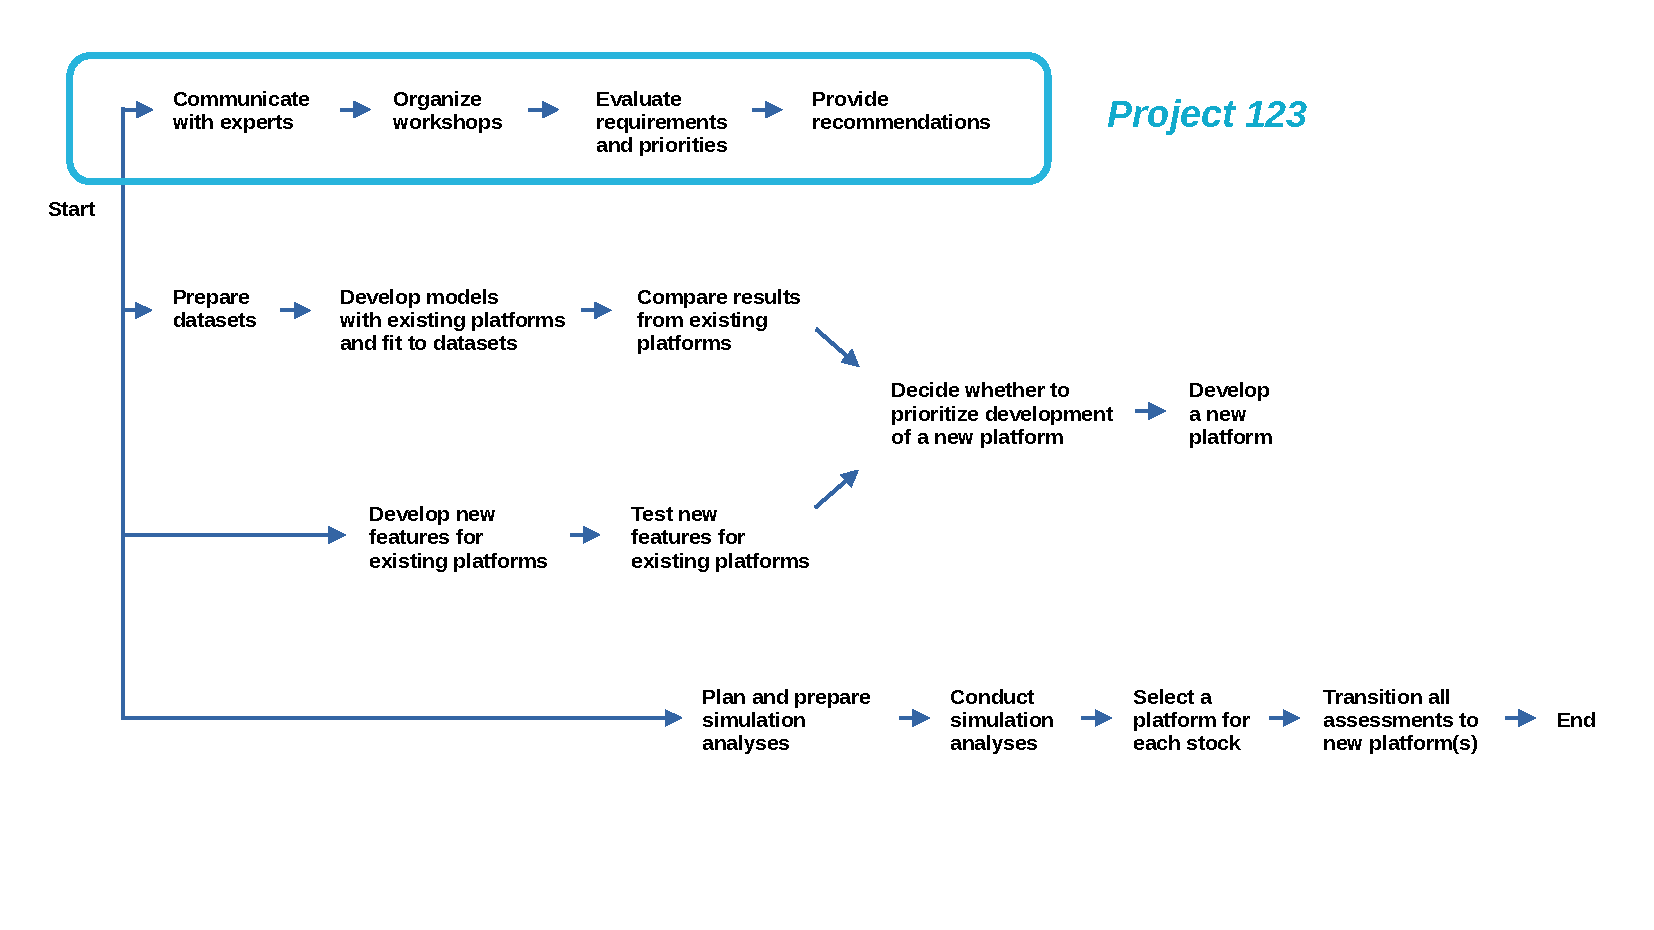
\includegraphics[width=0.95\paperwidth]{tasks}};
  \end{tikzpicture}
\end{frame}

% ______________________________________________________________________________

\begin{frame}{Possible Outcomes}\small
  If commitment and funding is limited, then the following unwanted outcome,\\
  characterized by a lack of progress, could well occur...\\[2ex]
  \textit{Upcoming assessments:}
  \begin{itemize}
    \item[] {\bf 2024} MFCL with config changes, other platform(s) did not work
    well, workshop
    \item[] {\bf 2025} MFCL with config changes, other platform(s) did not work
    well, workshop
    \item[] {\bf 2026} MFCL without config changes, other platform(s) did not
    work well, workshop
    \item[] {\bf 2027} MFCL without config changes, other platform(s) did not
    work well, workshop
    \item[] {\bf 2028} MFCL without config changes, other platform(s) did not
    work well, workshop
    \item[] {\bf 2029} MFCL without config changes, other platform(s) did not
    work well, workshop
    \item[] {\bf 2030} MFCL without config changes, other platform(s) did not
    work well, workshop
  \end{itemize}
\end{frame}

% ______________________________________________________________________________

\begin{frame}{Possible Outcomes}\small
  will depend on:\\[3ex]
  \textbf{Level of funding}
  \begin{itemize}
    \item[] \textgreen{Level 0} ~--~ Annual workshops, coordination\\[-1ex]
    \item[] \textgreen{Level 1} ~--~ Hire one person for 5 years\\[-1ex]
    \item[] \textgreen{Level 2} ~--~ Hire two people for 5 years\\[5ex]
  \end{itemize}
  \textbf{Partnerships}
  \begin{itemize}
    \item[] Tuna RFMOs ~--~ funding and scientists' time\\[-1ex]
    \item[] Domain experts in state-space model development ~--~ scientists'
    time\\[-1ex]
    \item[] Other funding sources\\[1ex]
  \end{itemize}
\end{frame}

% ______________________________________________________________________________

\begin{frame}{Summary}
  \begin{itemize}
    \item[] {\bf\darkblue Project P123} \comment{objective, background,
      terms of reference}\\[5ex]
    \item[] {\bf\darkblue Software Platforms} \comment{operational, current and
      future development}\\[5ex]
    \item[] {\bf\darkblue Road Ahead} \comment{assessments, workshops,
      collaboration, adaptive plan}\\[5ex]
    \item[] {\bf\darkblue Possible Outcomes} \comment{level of funding,
      partnerships}\\[1ex]
  \end{itemize}
\end{frame}

\end{document}
